\documentclass[border=2pt]{standalone}
\usepackage{pgfmath}
\usepackage{tikz}
\usetikzlibrary{shapes}
\usetikzlibrary{arrows.meta}
\usetikzlibrary{positioning}
\usetikzlibrary{calc}

\renewcommand\familydefault{\sfdefault}
\sffamily

\tikzset{
  pics/table/.style args = {#1/#2/#3}{
    code = {
      \begin{scope}
        \node [font=\scriptsize\ttfamily] at (1.5,0) {#1};
        \node [anchor=west, font=\scriptsize\ttfamily] at (0,-0.475) {id};
        \node (-id-w) [inner sep=0pt] at (0, -0.5) {};
        \node (-id-e) [inner sep=0pt] at (3, -0.5) {};
        \draw (0,0.25) rectangle (3,-0.25);
        \draw (0,-0.25) rectangle (3, -0.675);
        \draw (0,-0.675) rectangle (3,-0.8 - 0.25 * #3);
        \foreach[count=\i] \argtext in {#2} {
          \node [anchor=west,font=\scriptsize\ttfamily] at (0,-\i * 0.25 - 0.625) {\argtext};
          \node (-\i-w) [inner sep=0pt] at (0,-\i * 0.25 - 0.625) {};
          \node (-\i-e) [inner sep=0pt] at (3,-\i * 0.25 - 0.625) {};
          \node (-\i-w-inner) [inner sep=0pt] at (0.1,-\i * 0.25 - 0.625) {};
          \node (-\i-e-inner) [inner sep=0pt] at (2.9,-\i * 0.25 - 0.625) {};
        }
      \end{scope}
      \node (-center) [inner sep=0pt] at (1.5,-0.3 - #3 * 0.125) {};
      \node (-nw) [inner sep=0pt] at (0,0.25) {};
      \node (-ne) [inner sep=0pt] at (3,0.25) {};
      \node (-sw) [inner sep=0pt] at (0,-0.8 - #3 * 0.25) {};
      \node (-se) [inner sep=0pt] at (3,-0.8 - #3 * 0.25) {};
    }
  },
  pics/table with uuid/.style args = {#1/#2/#3}{
    code = {
      \begin{scope}
        \node [font=\scriptsize\ttfamily] at (1.5,0) {#1};
        \node [anchor=west, font=\scriptsize\ttfamily] at (0,-0.475) {uuid};
        \node (-uuid-w) [inner sep=0pt] at (0, -0.5) {};
        \node (-uuid-e) [inner sep=0pt] at (3, -0.5) {};
        \draw (0,0.25) rectangle (3,-0.25);
        \draw (0,-0.25) rectangle (3, -0.675);
        \draw (0,-0.675) rectangle (3,-0.8 - 0.25 * #3);
        \foreach[count=\i] \argtext in {#2} {
          \node [anchor=west,font=\scriptsize\ttfamily] at (0,-\i * 0.25 - 0.625) {\argtext};
          \node (-\i-w) [inner sep=0pt] at (0,-\i * 0.25 - 0.625) {};
          \node (-\i-e) [inner sep=0pt] at (3,-\i * 0.25 - 0.625) {};
          \node (-\i-w-inner) [inner sep=0pt] at (0.1,-\i * 0.25 - 0.625) {};
          \node (-\i-e-inner) [inner sep=0pt] at (2.9,-\i * 0.25 - 0.625) {};
        }
      \end{scope}
      \node (-center) [inner sep=0pt] at (1.5,-0.3 - #3 * 0.125) {};
      \node (-nw) [inner sep=0pt] at (0,0.25) {};
      \node (-ne) [inner sep=0pt] at (3,0.25) {};
      \node (-sw) [inner sep=0pt] at (0,-0.8 - #3 * 0.25) {};
      \node (-se) [inner sep=0pt] at (3,-0.8 - #3 * 0.25) {};
    }
  },
  pics/table without id/.style args = {#1/#2/#3}{
    code = {
      \begin{scope}
        \node [font=\scriptsize\ttfamily] at (1.5,0) {#1};
        \draw (0,0.25) rectangle (3,-0.25);
        \draw (0,-0.25) rectangle (3,-0.5 - 0.25 * #3);
        \foreach[count=\i] \argtext in {#2} {
          \node [anchor=west,font=\scriptsize\ttfamily] at (0,-\i * 0.25 - 0.25) {\argtext};
          \node (-\i-w) [inner sep=0pt] at (0,-\i * 0.25 - 0.25) {};
          \node (-\i-e) [inner sep=0pt] at (3,-\i * 0.25 - 0.25) {};
          \node (-\i-w-inner) [inner sep=0pt] at (0.1,-\i * 0.25 - 0.25) {};
          \node (-\i-e-inner) [inner sep=0pt] at (2.9,-\i * 0.25 - 0.25) {};
        }
      \end{scope}
    }
  },
  myarrow/.style = {
    Diamond[open]-Latex[],
    rounded corners=1mm
  },
  weak reference/.style = {
    Circle[open]-Latex[],
  },
  one to many/.style = {
    {Rays[n=6,length=1.2mm,width=1.2mm]}-Latex[],
  },
}

\begin{document}
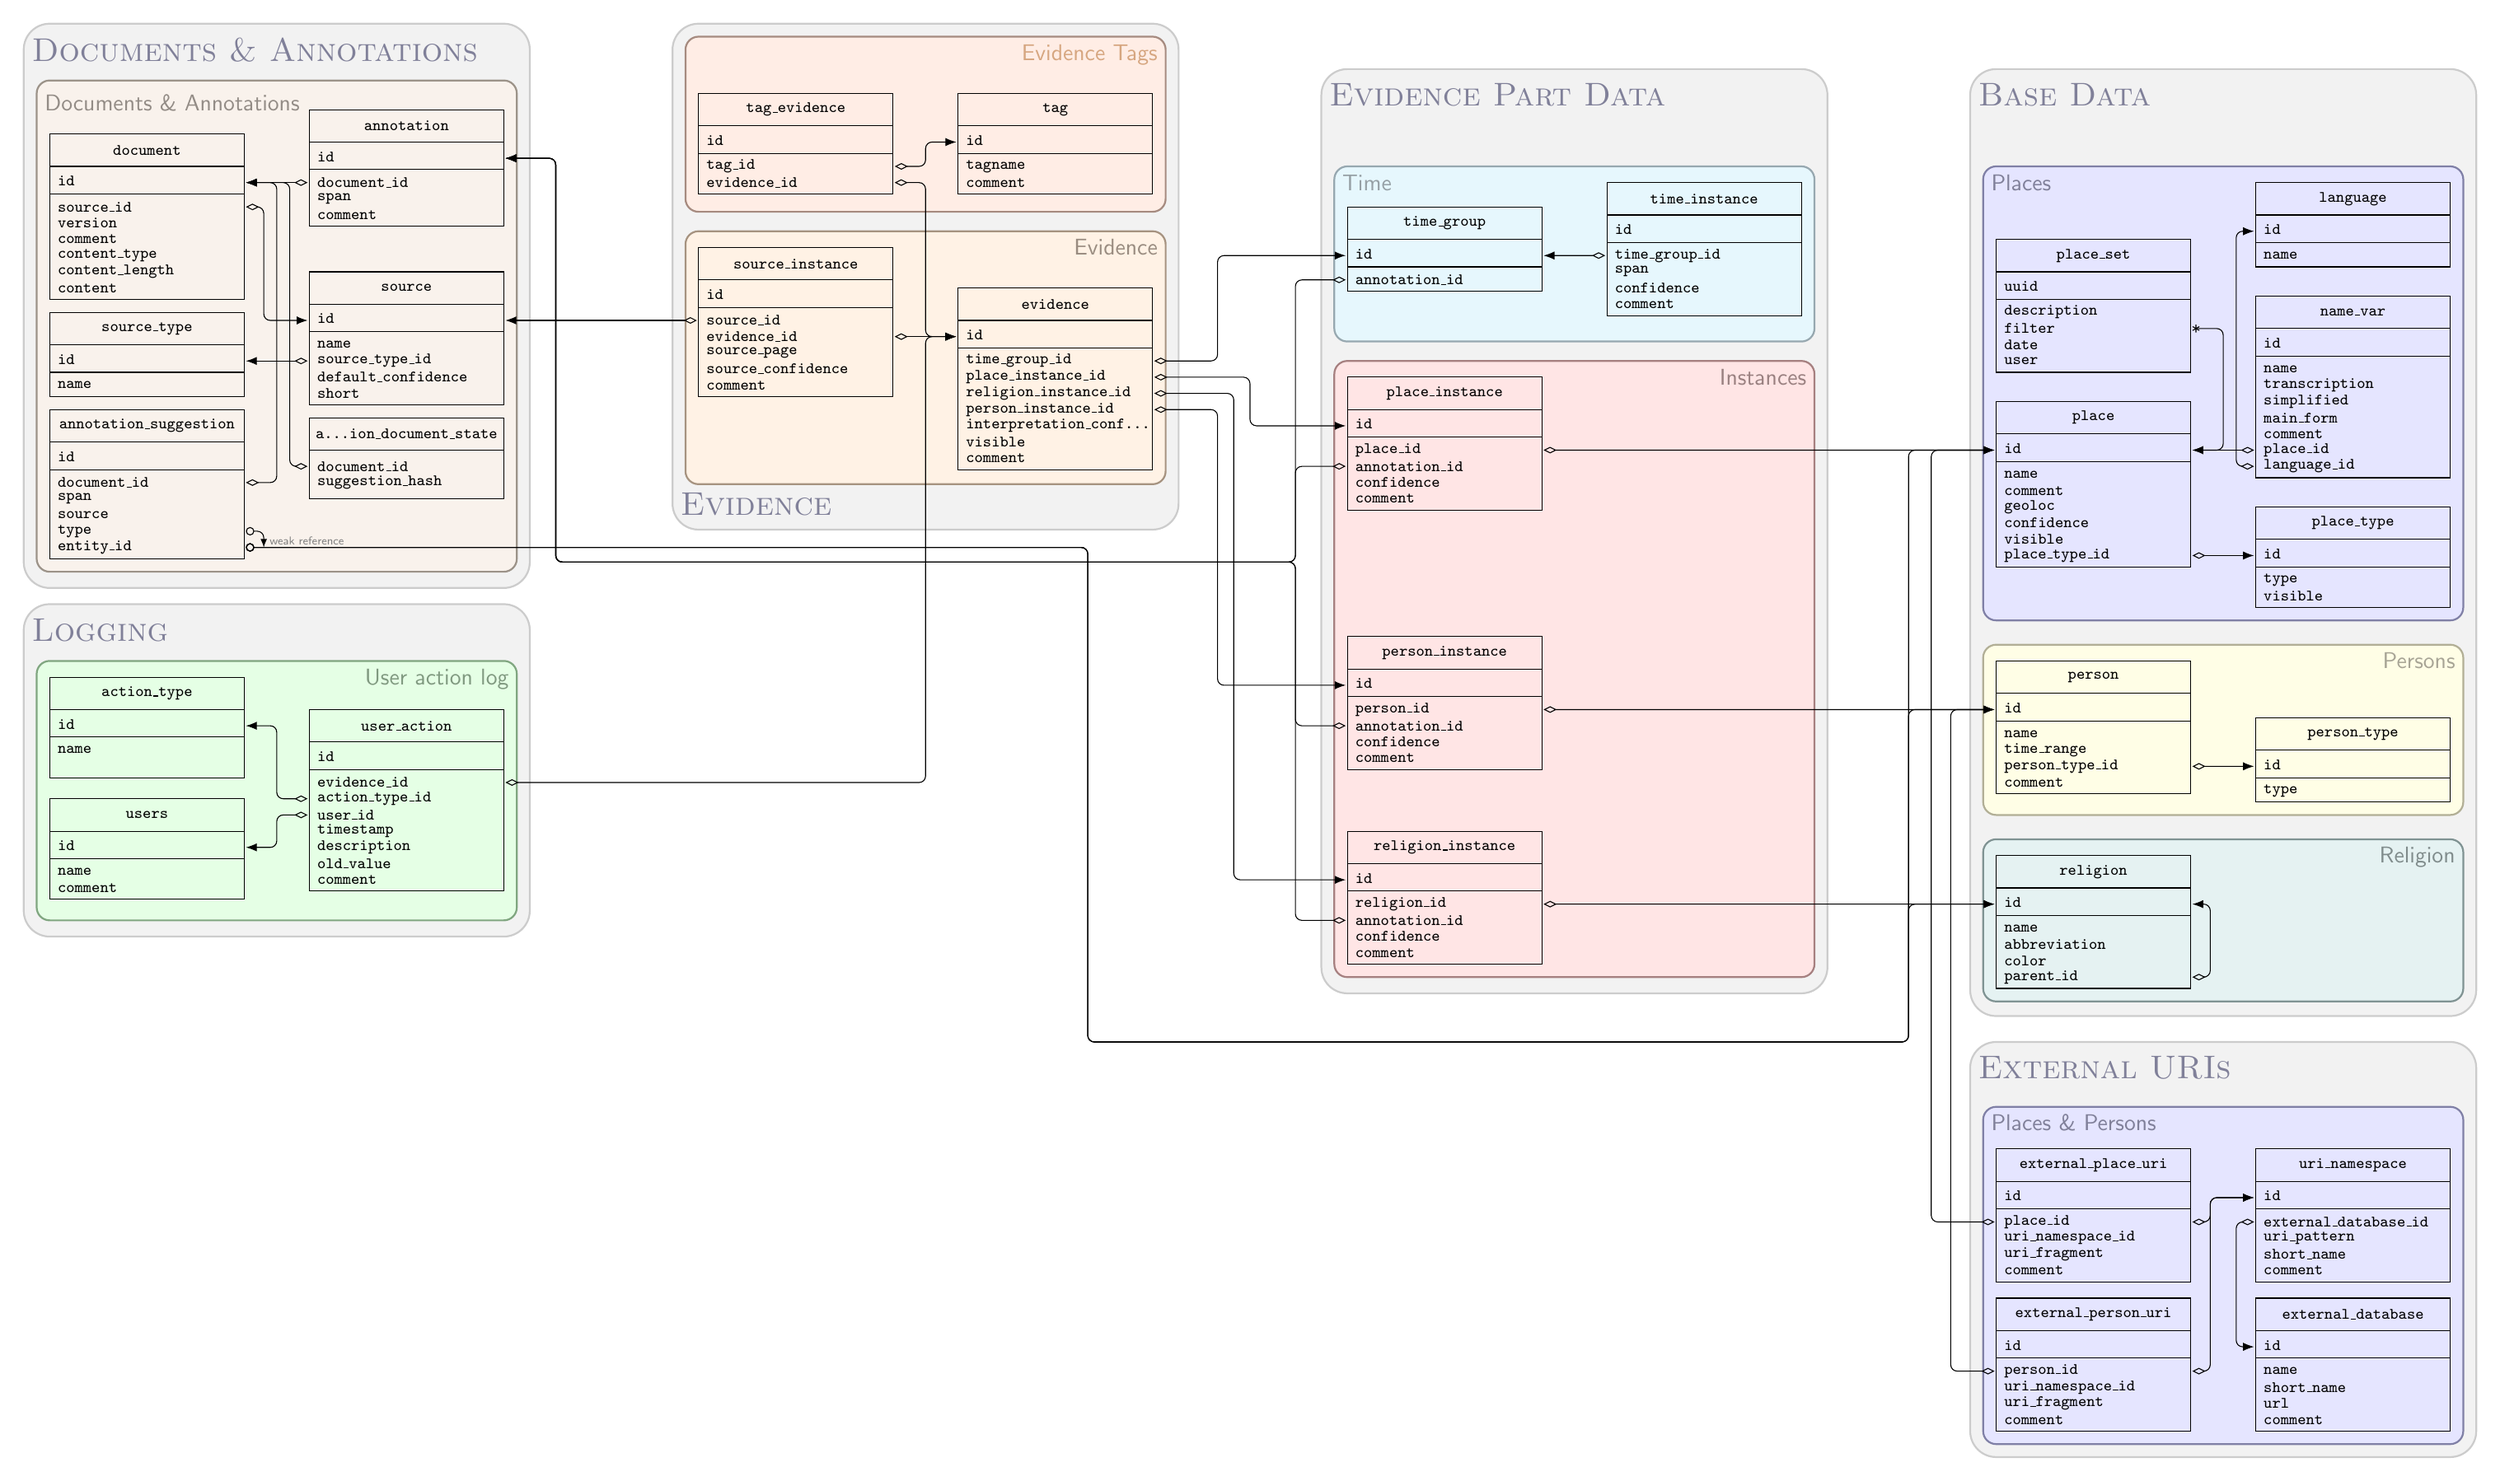
\begin{tikzpicture}
  %%%         DOCUMENTS AND ANNOTATIONS
  \begin{scope}[xshift=-6cm]
    \draw [thick,fill=black!5,draw=black!20,rounded corners=4mm] (-0.4,15.7) rectangle (7.4, 7);
    \node [anchor=north west,draw=none,text=black!80!blue!50] at (-0.4,15.6) {\Large\textsc{Documents \& Annotations}};

    \begin{scope}[yshift=11.625cm]
      \draw [thick,fill=brown!10,draw=brown!30!black!50,rounded corners=2mm] (-0.2,3.2) rectangle (7.2,-4.375);
      \node [anchor=north west,draw=none,text=black!80!brown!50] at (-0.2,3.1) {Documents \& Annotations};

      \pic (source) at (4,0)
      {table=source/{{name},{source\_type\_id},{default\_confidence},{short}}/4};
      \pic (source_type) at (0,-0.625)
      {table=source\_type/{{name}}/1};
      \pic (document) at (0,2.125)
      {table=document/{{source\_id},{version},{comment},{content\_type},{content\_length},{content}}/6};
      \pic (annotation) at (4,2.5)
      {table=annotation/{{document\_id},{span},{comment}}/3};

      \pic (annotation_suggestion) at (0,-2.125)
      {table=annotation\_suggestion/{{document\_id},{span},{source},{type},{entity\_id}}/5};
      \pic (annotation_suggestion_document_state) at (4,-2.25)
      {table without id=a...ion\_document\_state/{{document\_id},{suggestion\_hash}}/2};

      \draw [myarrow] (source-2-w) -- (source_type-id-e);
      \draw [myarrow] (document-1-e) -- ++(0.3,0) |- (source-id-w);
      \draw [myarrow] (annotation-1-w) -- (document-id-e);

      \draw [myarrow] (annotation_suggestion-1-e) -- ++(0.5,0) |- (document-id-e);
      \draw [myarrow] (annotation_suggestion_document_state-1-w) -- ++(-0.3,0) |- (document-id-e);
    \end{scope}
  \end{scope}

  \begin{scope}[xshift=-6cm,yshift=-2.25cm]
    \draw [thick,fill=black!5,draw=black!20,rounded corners=4mm] (-0.4,9) rectangle (7.4, 3.875);
    \node [anchor=north west,draw=none,text=black!80!blue!50] at (-0.4,8.9) {\Large\textsc{Logging}};

    %%%         USER ACTION LOGGING
    \begin{scope}[yshift=6.625cm]
      \draw [thick,fill=green!10,draw=green!30!black!50,rounded corners=2mm] (-0.2,-2.5) rectangle (7.2,1.5);
      \node [anchor=north east,draw=none,text=black!80!green!50] at (7.2,1.5) {User action log};

      \pic (user_action) at (4, 0.5) {table=user\_action/{{evidence\_id},{action\_type\_id},{user\_id},{timestamp},{description},{old\_value},{comment}}/7};
      \pic (users) at (0,-0.875) {table=users/{{name},{comment}}/2};
      \pic (action_type) at (0, 1) {table=action\_type/{{name}}/2};

      \draw [myarrow] (user_action-3-w) -- ++(-0.5,0) |- (users-id-e);
      \draw [myarrow] (user_action-2-w) -- ++(-0.5,0) |- (action_type-id-e);
    \end{scope}

  \end{scope}

  %%%         EVIDENCE
  \begin{scope}[xshift=4cm]
    \draw [thick,fill=black!5,draw=black!20,rounded corners=4mm] (-0.4,15.7) rectangle (7.4, 7.9);
    \node [anchor=south west,draw=none,text=black!80!blue!50] at (-0.4,8) {\Large\textsc{Evidence}};

    \begin{scope}[yshift=15cm]
      \draw [thick,fill=red!40!orange!10,draw=red!40!orange!30!black!50,rounded corners=2mm] (-0.2,0.5) rectangle (7.2,-2.2);
      \node [anchor=north east,draw=none,text=black!80!red!40!orange!50] at (7.2,0.5) {Evidence Tags};

      \pic (tag) at (4,-0.625)
      {table=tag/{{tagname},{comment}}/2};
      \pic (tag_evidence) at (0,-0.625)
      {table=tag\_evidence/{{tag\_id},{evidence\_id}}/2};

      \draw [myarrow] (tag_evidence-1-e) -- ++(0.5,0) |- (tag-id-w);
    \end{scope}

    \begin{scope}[yshift=12cm]
      \draw [thick,fill=orange!10,draw=orange!30!black!50,rounded corners=2mm] (-0.2,0.5) rectangle (7.2,-3.4);
      \node [anchor=north east,draw=none,text=black!80!orange!50] at (7.2,0.5) {Evidence};

      \pic (evidence) at (4,-0.625)
      {table=evidence/{{time\_group\_id},{place\_instance\_id},{religion\_instance\_id},{person\_instance\_id},{interpretation\_conf\dots},{visible},{comment}}/7};
      \pic (source_instance) at (0,0)
      {table=source\_instance/{{source\_id},{evidence\_id},{source\_page},{source\_confidence},{comment}}/5};

      \draw [myarrow] (source_instance-2-e) -- (evidence-id-w);
    \end{scope}

    \draw [myarrow] (tag_evidence-2-e) -- ++(0.5,0) |- (evidence-id-w);
  \end{scope}

  %%%         EVIDENCE PART DATA
  \begin{scope}[xshift=14cm]
    \draw [thick,fill=black!5,draw=black!20,rounded corners=4mm] (-0.4,15) rectangle (7.4, 0.75);
    \node [anchor=north west,draw=none,text=black!80!blue!50] at (-0.4,14.9) {\Large\textsc{Evidence Part Data}};

    %%%         TIME
    \begin{scope}[yshift=13cm]
      \draw [thick,fill=cyan!10,draw=cyan!30!black!50,rounded corners=2mm] (-0.2,0.5) rectangle (7.2,-2.2);
      \node [anchor=north west,draw=none,text=black!80!cyan!50] at (-0.2,0.5) {Time};

      \pic (time_instance) at (4,0)
      {table=time\_instance/{{time\_group\_id},{span},{confidence},{comment}}/4};
      \pic (time_group) at (0,-0.375)
      {table=time\_group/{{annotation\_id}}/1};

      \draw [myarrow] (time_instance-1-w) -- (time_group-id-e);
    \end{scope}

    %           PLACE_INSTANCE
    \begin{scope}[yshift=10cm]
      \draw [thick,fill=red!10,draw=red!30!black!50,rounded corners=2mm] (-0.2,0.5) rectangle (7.2,-9);
      \node [anchor=north east,draw=none,text=black!80!red!50] at (7.2,0.5) {Instances};

      \pic (place_instance) at (0,0)
      {table=place\_instance/{{place\_id},{annotation\_id},{confidence},{comment}}/4};
      \pic (person_instance) at (0,-4)
      {table=person\_instance/{{person\_id},{annotation\_id},{confidence},{comment}}/4};
      \pic (religion_instance) at (0,-7)
      {table=religion\_instance/{{religion\_id},{annotation\_id},{confidence},{comment}}/4};

    \end{scope}


  \end{scope}

  %%%         EVIDENCE BASE DATA
  \begin{scope}[xshift=24cm]

    \draw [thick,fill=black!5,draw=black!20,rounded corners=4mm] (-0.4,15) rectangle (7.4, 0.4);
    \node [anchor=north west,draw=none,text=black!80!blue!50] at (-0.4,14.9) {\Large\textsc{Base Data}};

    %%%         PLACE DATA
    \begin{scope}[yshift=9cm]
      \draw [thick,fill=blue!10,draw=blue!30!black!50,rounded corners=2mm] (-0.2,4.5) rectangle (7.2,-2.5);
      \node [anchor=north west,draw=none,text=black!80!blue!50] at (-0.2,4.5) {Places};

      \pic (place) at (0,0.625)
      { table=place/{{name},{comment},{geoloc},{confidence},{visible},{place\_type\_id}}/6 };
      \pic (place_type) at (4,-1)
      { table=place\_type/{{type},{visible}}/2 };
      \pic (name_var) at (4,2.25)
      { table=name\_var/{{name},{transcription},{simplified},{main\_form},{comment},{place\_id},{language\_id}}/7 };
      \pic (language) at (4,4)
      { table=language/{{name}}/1 };
      \pic (place_set) at (0,3.125)
      { table with uuid=place\_set/{{description},{filter},{date},{user}}/4};

      \draw [myarrow] (place-6-e) -- (place_type-id-w);
      \draw [myarrow] (name_var-6-w) -- (place-id-e);
      \draw [myarrow] (name_var-7-w) -- ++(-0.3,0) |- (language-id-w);
      \draw [myarrow,one to many] (place_set-2-e) -- ++(0.5,0) |- (place-id-e);
    \end{scope}

    %%%          PERSONS
    \begin{scope}[yshift=3.625cm]
      \draw [thick,fill=yellow!10,draw=yellow!30!black!50,rounded corners=2mm] (-0.2,2.5) rectangle (7.2,-0.125);
      \node [anchor=north east,draw=none,text=black!80!yellow!50] at (7.2,2.5) {Persons};

      \pic (person) at (0,2)
      {table=person/{{name},{time\_range},{person\_type\_id},{comment}}/4};
      \pic (person_type) at (4,1.125)
      {table=person\_type/{{type}}/1};

      \draw [myarrow] (person-3-e) -- (person_type-id-w);
    \end{scope}

    %%%         RELIGION
    \begin{scope}[yshift=2.625cm]
      \draw [thick,fill=teal!10,draw=teal!30!black!50,rounded corners=2mm] (-0.2,0.5) rectangle (7.2,-2);
      \node [anchor=north east,draw=none,text=black!80!teal!50] at (7.2,0.5) {Religion};

      \pic (religion) at (0,0)
      {table=religion/{{name},{abbreviation},{color},{parent\_id}}/4};

      \draw [myarrow] (religion-4-e) -- ++(0.3,0) |- (religion-id-e);
    \end{scope}

  \end{scope}

  %%%         EXTERNAL URIs
  \begin{scope}[xshift=24cm]

    \draw [thick,fill=black!5,draw=black!20,rounded corners=4mm] (-0.4,0) rectangle (7.4, -6.4);
    \node [anchor=north west,draw=none,text=black!80!blue!50] at (-0.4,-0.1) {\Large\textsc{External URIs}};

    %%%         PLACES AND PERSONS
    \begin{scope}[yshift=-6cm]
      \draw [thick,fill=blue!10,draw=blue!30!black!50,rounded corners=2mm] (-0.2,5) rectangle (7.2,-0.2);
      \node [anchor=north west,draw=none,text=black!80!blue!50] at (-0.2,5) {Places \& Persons};

      \pic (external_database) at (4,1.8)
      { table=external\_database/{{name},{short\_name},{url},{comment}}/4 };
      \pic (uri_namespace) at (4,4.1)
      { table=uri\_namespace/{{external\_database\_id},{uri\_pattern},{short\_name},{comment}}/4 };
      \pic (external_place_uri) at (0,4.1)
      { table=external\_place\_uri/{{place\_id},{uri\_namespace\_id},{uri\_fragment},{comment}}/4 };
      \pic (external_person_uri) at (0,1.8)
      { table=external\_person\_uri/{{person\_id},{uri\_namespace\_id},{uri\_fragment},{comment}}/4 };

      \draw [myarrow] (uri_namespace-1-w) -- ++(-0.3,0) |- (external_database-id-w);
      \draw [myarrow] (external_place_uri-1-e) -- ++(0.3,0) |- (uri_namespace-id-w);
      \draw [myarrow] (external_person_uri-1-e) -- ++(0.3,0) |- (uri_namespace-id-w);
    \end{scope}
  \end{scope}

  %%%         INTER-PLACE LINKS
  \draw [myarrow] (place_instance-1-e) -- (place-id-w);
  \draw [myarrow] (person_instance-1-e) -- (person-id-w);
  \draw [myarrow] (religion_instance-1-e) -- (religion-id-w);

  \draw [myarrow] (evidence-1-e) -- ++(1,0) |- (time_group-id-w);
  \draw [myarrow] (evidence-2-e) -- ++(1.5,0) |- (place_instance-id-w);
  \draw [myarrow] (evidence-3-e) -- ++(1.25,0) |- (religion_instance-id-w);
  \draw [myarrow] (evidence-4-e) -- ++(1,0) |- (person_instance-id-w);

  \draw [myarrow] (source_instance-1-w) -- (source-id-e);

  \coordinate (to-annotation-middlestep) at (10, 7.4);
  \coordinate (annotation-id-e-outer) at ($ (annotation-id-e) + (0.8,0) $);
  \draw [myarrow] (time_group-1-w) -- ++(-0.8,0) |- (to-annotation-middlestep)-| (annotation-id-e-outer) -- (annotation-id-e);
  \draw [myarrow] (place_instance-2-w) -- ++(-0.8,0) |- (to-annotation-middlestep) -| (annotation-id-e-outer) -- (annotation-id-e);
  \draw [myarrow] (religion_instance-2-w) -- ++(-0.8,0) |- (to-annotation-middlestep) -| (annotation-id-e-outer) -- (annotation-id-e);
  \draw [myarrow] (person_instance-2-w) -- ++(-0.8,0) |- (to-annotation-middlestep) -| (annotation-id-e-outer) -- (annotation-id-e);

  \coordinate (to-entities-middlestep) at (10,0);
  \draw [myarrow,weak reference] (annotation_suggestion-5-e) -| (to-entities-middlestep) -| ($ (place-id-w) + (-1.35,0) $) -- (place-id-w);
  \draw [myarrow,weak reference] (annotation_suggestion-5-e) -| (to-entities-middlestep) -| ($ (person-id-w) + (-1.35,0) $) -- (person-id-w);
  \draw [myarrow,weak reference] (annotation_suggestion-5-e) -| (to-entities-middlestep) -| ($ (religion-id-w) + (-1.35,0) $) -- (religion-id-w);
  \coordinate (weak-reference-label) at ($ (annotation_suggestion-5-e) + (0.3,0) $);
  \node [anchor=south west,color=gray,inner sep=1,xshift=0.5mm] at (weak-reference-label) { \tiny weak reference };
  \draw [rounded corners=1mm,{Circle[open]}-{Latex[width=1mm,length=1.3mm]}] (annotation_suggestion-4-e) -| (weak-reference-label);

  \draw [myarrow] (user_action-1-e) -- ++(6.5,0) |- (evidence-id-w);

  \draw [myarrow] (external_place_uri-1-w) -- ++(-1.0,0) |- (place-id-w);
  \draw [myarrow] (external_person_uri-1-w) -- ++(-0.7,0) |- (person-id-w);
\end{tikzpicture}
\end{document}
